\documentclass[10pt]{article}
\usepackage{neurips_2026}

% Core packages
\usepackage[utf8]{inputenc}
\usepackage[T1]{fontenc}
\usepackage{hyperref}
\usepackage{url}
\usepackage{booktabs}
\usepackage{amsfonts}
\usepackage{amsmath}
\usepackage{amsthm}
\newtheorem{definition}{Definition}
\usepackage{nicefrac}
\usepackage{microtype}
\usepackage{graphicx}
\usepackage{xcolor}
\usepackage{multirow}
\usepackage{array}
\usepackage{subcaption}
\usepackage{enumitem}
\usepackage{xspace}
\usepackage{tabularx}
\usepackage{colortbl}

% NeurIPS checklist answer commands
\newcommand{\answerYes}[1][]{{\bf Yes.} #1}
\newcommand{\answerNo}[1][]{{\bf No.} #1}
\newcommand{\answerNA}[1][]{{\bf N/A.} #1}

% Custom commands
\newcommand{\epikg}{EpiKG\xspace}
\newcommand{\ie}{i.e.,\xspace}
\newcommand{\eg}{e.g.,\xspace}
\newcommand{\cf}{cf.\xspace}
\newcommand{\pp}{\,\text{pp}}
\newcommand{\ci}[2]{[#1, #2]}
\newcommand{\smark}{\textcolor{green!60!black}{\checkmark}}
\newcommand{\xmark}{\textcolor{red!80!black}{$\times$}}

% For double-blind
\hypersetup{
  colorlinks=true,
  linkcolor=blue!60!black,
  citecolor=blue!60!black,
  urlcolor=blue!60!black,
  pdfborder={0 0 0}
}

\title{EpiKG: End-to-End Epistemic Preservation in Clinical Knowledge Graphs for Assertion-Aware Retrieval-Augmented Generation}

\author{
  Anonymous Author(s)
}

\begin{document}

\maketitle

% ============================================================
% ABSTRACT
% ============================================================
\begin{abstract}
% Abstract
% NOTE: \begin{abstract} and \end{abstract} are in main.tex

Clinical NLP systems can detect assertion status---negation, uncertainty, family history---with high accuracy, yet to our knowledge no existing system preserves this epistemic metadata through knowledge graph construction to retrieval-augmented generation.
This \emph{epistemic propagation gap} causes RAG systems to conflate mentioned conditions with present ones, retrieving ``patient denies diabetes'' as evidence of diabetes.
We present EpiKG, a clinical knowledge graph system that preserves assertion status end-to-end through a 7-value assertion schema, a tri-temporal edge model with Allen's interval algebra, shared concept nodes with cross-patient assertion statistics, and an assertion-aware GraphRAG pipeline.
We introduce two benchmarks on MIMIC-IV data: ClinicalBench (400 assertion-sensitive questions across 9 epistemic categories) and Slice Bench (144 longitudinal questions across 3 patient complexity tiers).
On ClinicalBench, vanilla RAG \emph{degrades} LLM accuracy by 10.7 percentage points (73.2\%$\rightarrow$62.5\%), while epistemic KG-RAG recovers to 71.5\% with a different category profile---gaining on family history (+70\,pp) and uncertainty (+7.5\,pp) but losing on duration ($-$46.7\,pp) and conditional ($-$35\,pp)---and achieves higher clinical safety scores (0.775 vs.\ 0.765).
On Slice Bench, preliminary tier-stratified results suggest the KG benefit concentrates in high-complexity patients (+5.0\,pp for 15+ encounters vs.\ +0.6\,pp for 1--2), though per-tier samples are small ($n=2$ patients each).
Cross-model validation on ClinicalBench (Claude Opus 4.6) reveals a model-strength interaction: epistemic KG-RAG produces a $+9.0\pp$ gain for MedGemma~27B but a $-2.2\pp$ regression for Opus, suggesting that structured epistemic evidence is most valuable when the LLM lacks sufficient parametric knowledge to reason about assertion status independently.
These results suggest that structured epistemic context is most valuable when document volume overwhelms simple retrieval or model capability is limited, and that assertion-blind knowledge graphs can be worse than no graph at all.

\end{abstract}

% ============================================================
% 1. INTRODUCTION
% ============================================================
\section{Introduction}
\label{sec:intro}
% Section 1: Introduction
% NOTE: \section{Introduction} and \label{sec:intro} are in main.tex

A physician documents ``patient denies chest pain, sister had MI at 45, will consider statin if lipids remain elevated''---a single sentence encoding four epistemic states: a negated symptom, a family-history event, a hypothetical action, and an implicit present condition.
Clinical NLP can detect these assertions accurately~\cite{uzuner2011i2b2assertion, gul2025beyondnegation}, yet when a RAG system ingests the same note, assertion context is flattened: negation is lost, family attribution collapses onto the patient, and downstream reasoning may conclude the patient \emph{has} chest pain and \emph{had} an MI.
We call this the \emph{epistemic propagation gap}---the systematic loss of assertion status as clinical information moves from extraction through storage to retrieval.

The gap persists because, to our knowledge, prior KG-RAG systems do not propagate assertion labels beyond the extraction stage into graph-augmented retrieval.
Clinical NLP pipelines (cTAKES, John Snow Labs) detect assertions, but do not carry them as edge attributes into knowledge graph construction or retrieval.
OMOP excludes negated conditions from \texttt{CONDITION\_OCCURRENCE}~\cite{omop2024}; FHIR provides \texttt{verificationStatus} for \texttt{Condition} resources only, covering a fraction of the clinical data model.
Graph-augmented RAG systems---GraphRAG~\cite{edge2024graphrag}, GFM-RAG~\cite{luo2025gfmrag}, KARE~\cite{jiang2025kare}, Medical-Graph-RAG~\cite{wu2025medicalgraphrag}---build KGs that discard the metadata distinguishing ``patient has diabetes'' from ``rule out diabetes.''
Similarly, recent clinical QA systems---MedPaLM~2~\cite{singhal2023medpalm2}, Med-Gemini~\cite{saab2024medgemini}, AMIE~\cite{tu2024amie}---excel at medical knowledge recall but are not designed for longitudinal assertion reasoning over real patient records, which is the gap ClinicalBench targets.
A parallel \emph{temporal integration gap} exists: clinical events span three time dimensions (valid time, transaction time, NLP-asserted temporality), yet existing systems model at most two~\cite{huang2024medtkg,ramirez2025graphiti}.

We present \epikg, a clinical KG-RAG system that preserves epistemic status end-to-end, and ClinicalBench, a 400-question benchmark that exposes the propagation gap.
Our contributions are primarily \emph{empirical findings and a design principle}, not system components:

\begin{enumerate}[leftmargin=*, topsep=4pt, itemsep=2pt]
  \item \textbf{The epistemic propagation gap.} We identify and formalize the systematic loss of assertion metadata across clinical NLP pipelines, derive an information-theoretic loss bound (Section~\ref{sec:system:formal}, Appendix~\ref{app:formal}), and implement end-to-end preservation as a testable invariant.

  \item \textbf{Assertions alone do not help; routing is the active ingredient.} Adding assertion metadata to graph edges without question-type-specific retrieval does not improve accuracy ($-3.2\pp$, C3$\to$C4; CI crossing zero, $p = 0.37$). The entire C3$\to$C4g gain ($+19.0\pp$) is attributable to intent-aware routing ($+22.2\pp$, C4$\to$C4g; $p < 10^{-10}$). Metadata enrichment without retrieval alignment is insufficient.

  \item \textbf{Knowledge-compensator pattern.} Across four models from distinct training lineages, models with weaker baselines gain more from KG-RAG, and all converge to 57.5--69.0\% under C4g despite C1 baselines spanning 20.5\% to 37.0\%. This convergence pattern---observed descriptively across four data points---is consistent with the epistemic KG providing a knowledge floor that partially compensates for model-specific weaknesses.

  \item \textbf{ClinicalBench.} A 400-question benchmark across 9 assertion-sensitive categories (negation, uncertainty, conditional, family history, sequence, current state, duration, historical, change) that exposes category$\times$condition interactions invisible to aggregate metrics. Released with Croissant metadata on HuggingFace.

  \item \textbf{A falsifiable design principle.} Preserve epistemic metadata \emph{and} route retrieval by question intent, then evaluate by category$\times$condition interaction rather than aggregate score. This is not a system architecture but a falsifiable constraint: any pipeline violating it should underperform on assertion-sensitive longitudinal QA.
\end{enumerate}

Our central research question is: \emph{under what conditions does structured epistemic context help, hurt, or break even relative to unstructured retrieval and no retrieval?}
The answer is interactional rather than uniform: gains depend on question type, routing policy, and model.
Intent-aware KG-RAG improves all nine ClinicalBench categories, with largest effects on cross-admission longitudinal tasks; assertions without routing do not improve temporal categories; and brute-force long context does not recover these failures despite a large token window.


% ============================================================
% 2. RELATED WORK
% ============================================================
\section{Related Work}
\label{sec:related}
% Section 2: Related Work
% NOTE: \section{Related Work} and \label{sec:related} are in main.tex

We organize prior work along four axes and synthesize the gaps that \epikg addresses (Table~\ref{tab:gap}, Appendix).

\paragraph{Medical RAG systems.}
Graph-augmented retrieval has emerged as a leading paradigm for medical QA.
GraphRAG~\cite{edge2024graphrag} introduced community-based summarization; GFM-RAG~\cite{luo2025gfmrag} trained an 8M-parameter graph foundation model across 60 KGs (14M+ triples); KARE~\cite{jiang2025kare} adapted community retrieval to clinical decision support; DoctorRAG~\cite{lu2025doctorrag} emulates physician reasoning; MedRAG~\cite{wang2025medrag} constructs hierarchical diagnostic KGs; Medical-Graph-RAG~\cite{wu2025medicalgraphrag} links documents via triple graphs.
Concurrent work addresses EHR-specific retrieval: EHR-RAG~\cite{cao2026ehrrag} evaluates retrieval strategies over structured EHR tables, and MediGRAF~\cite{thio2025medigraf} builds medical KGs via multi-agent extraction.
Yet no published medical RAG system models assertion status or temporal context; GFM-RAG and KARE build population-level graphs rather than patient-level graphs from clinical text, and a recent survey~\cite{graphragsurvey2025} confirms no system incorporates epistemic metadata into the retrieval graph.

\paragraph{Clinical QA benchmarks and systems.}
Large-scale medical QA systems have advanced rapidly: MedPaLM~2~\cite{singhal2023medpalm2} reaches 86.5\% on MedQA-USMLE via ensemble refinement; Med-Gemini~\cite{saab2024medgemini} extends to multimodal clinical reasoning; AMIE~\cite{tu2024amie} achieves specialist-level diagnostic dialogue.
These systems target \emph{medical knowledge recall}---answering exam-style questions from parametric knowledge or medical literature.
ClinicalBench targets a complementary task: \emph{assertion-faithful longitudinal reasoning} over real EHR records, where the challenge is not knowing that metformin treats diabetes but knowing whether \emph{this patient} is still on metformin, whether a condition was ruled out or confirmed, and how the clinical picture changed across admissions.
EHR-specific QA benchmarks exist---emrQA~\cite{pampari2018emrqa} (1M+ question-answer pairs from clinical notes) and EHR-RAG~\cite{cao2026ehrrag} (structured EHR retrieval)---but neither evaluates assertion-sensitive reasoning or category$\times$condition interactions.

\paragraph{Clinical KG construction.}
Multi-LLM KG-RAG~\cite{chen2026multilllmkgrag} uses multi-agent LLM prompting with schema-constrained extraction for oncology, modeling uncertainty via entropy but not tracking assertion classes on edges.
AutoRD~\cite{li2024autord} applies GPT-4 to rare disease literature; RECAP-KG~\cite{remy2024recapkg} handles messy GP notes; FHIR-Ontop-OMOP~\cite{yun2022fhirontopomop} generates virtual KGs from OMOP data.
All share a common limitation: assertion status is not propagated into the final graph.

\paragraph{Assertion detection.}
NegEx~\cite{chapman2001negex} introduced trigger-based negation detection; ConText~\cite{harkema2009context} extended it with temporality and experiencer.
The i2b2/VA shared task~\cite{uzuner2011i2b2assertion} formalized a six-class taxonomy; Gul et al.~\cite{gul2025beyondnegation} fine-tuned LLMs to 0.962 accuracy.
All treat assertion detection as a terminal annotation task: labels are not carried into knowledge graphs or retrieval systems.

Assertion detection is necessary but not sufficient: labels must also be \emph{temporally situated}---the same condition may be present in one encounter and absent in the next.

\paragraph{Temporal knowledge graphs.}
MedTKG~\cite{huang2024medtkg} constructs temporal KGs with time-stamped snapshots (event time only); Graphiti~\cite{ramirez2025graphiti} implements bitemporal edges~\cite{snodgrass2000temporal} but lacks clinical ontology alignment; TEO~\cite{li2020teo} and TCL~\cite{ong2023tcl} formalize Allen's relations~\cite{allen1983temporal} as annotation ontologies or modal operators rather than KG edge attributes.
Uncertainty quantification in biomedical KGs~\cite{bao2024uncertaintybiomedkg} has not been connected to assertion taxonomies.
Two structural gaps emerge: an \emph{epistemic propagation gap} (assertion-detecting systems do not persist labels into KGs) and a \emph{temporal integration gap} (temporal formalisms operate as annotation layers, not as KG edge attributes participating in retrieval).
\epikg closes both by carrying assertion and temporal metadata as first-class properties through every pipeline stage.


% ============================================================
% 3. SYSTEM DESIGN
% ============================================================
\section{System Design}
\label{sec:system}
% Section 3: System Design

\subsection{Method Overview}
\label{sec:system:overview}

\epikg implements three key ideas: (1)~end-to-end epistemic preservation, carrying assertion labels from NLP extraction through OMOP mapping, fact construction, KG materialization, and retrieval; (2)~tri-temporal edge representation, storing valid time, transaction time, and NLP-asserted temporality on every KG edge; and (3)~intent-aware routing, matching graph traversal strategy to question type.
The first two ideas are necessary infrastructure; the third is where the performance gain originates.
The key invariant is that \textit{epistemic assertion status} is a first-class attribute at every stage, not an NLP annotation discarded after extraction (Figure~\ref{fig:architecture}).
Clinical concepts are stored once as shared global nodes; patient-specific semantics (assertion status, temporality, confidence) reside on edges.

\begin{figure}[t]
\centering
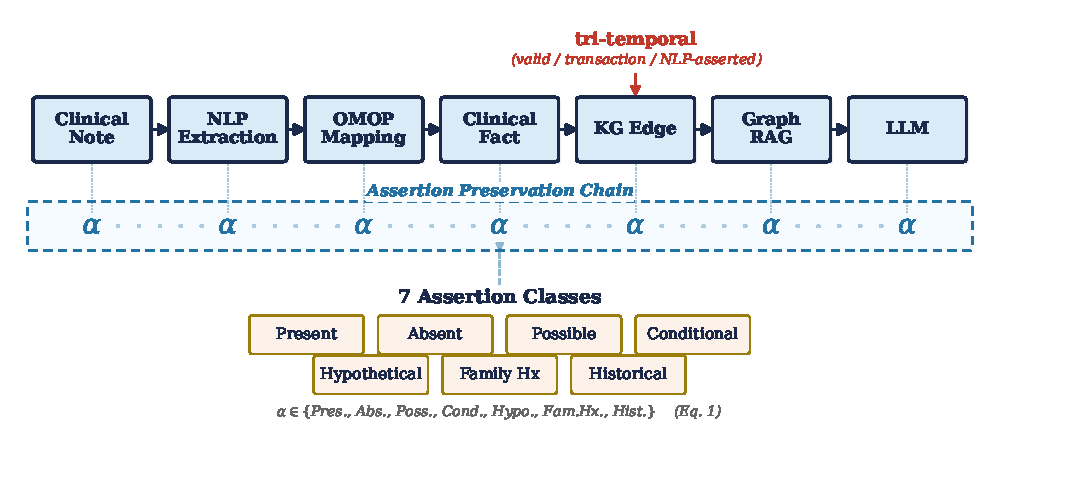
\includegraphics[width=\textwidth]{figures/fig1_architecture.pdf}
\caption{The \epikg pipeline. The assertion label $\alpha$ (highlighted) is preserved as a first-class attribute from NLP extraction through OMOP mapping, fact construction, KG materialization, and assertion-aware GraphRAG.}
\label{fig:architecture}
\end{figure}

\subsection{Epistemic Assertion Schema}
\label{sec:system:assertion}

\looseness=-1
Clinical notes abound with qualified statements---``\textit{no evidence of pneumonia},'' ``\textit{possible CHF},'' ``\textit{mother had breast cancer}''---yet standard representations discard these qualifiers.
OMOP excludes negated conditions entirely~\cite{omop2024}; FHIR limits assertion metadata to conditions.
\epikg defines a seven-value assertion taxonomy:
%
\begin{equation}
\label{eq:assertion}
\alpha \in \{\text{\scriptsize Pres., Abs., Poss., Cond., Hypo., Fam.Hx., Hist.}\}
\end{equation}
%
This extends the i2b2 six-class taxonomy~\cite{uzuner2011i2b2assertion} by separating \textsc{Historical} from \textsc{Family\_History}, a clinically important distinction that prior work conflates (definitions in Appendix~\ref{app:assertions}).
A rule-based classifier (122 scope-aware trigger patterns) assigns $\alpha$ with an associated confidence score.
The label is carried through every stage: from \texttt{ExtractedMention} through ensemble merging, \texttt{ClinicalFact} records, KG edge properties, and retrieval scoring.
Additionally, each edge carries a tri-temporal representation---valid time, transaction time, and NLP-asserted temporality---with Allen-style interval relations as first-class retrieval features (formalized in Appendix~\ref{app:temporal_model}).

\subsection{Formal Epistemic Preservation}
\label{sec:system:formal}

We formalize the epistemic invariant maintained by the \epikg pipeline, building on the ontological principle that aboutness must be preserved across transformations~\cite{ceusters2015ontologyepistemology}.
The \emph{epistemic state} of a clinical mention $m$ is the tuple $e(m) = (c, \alpha, \xi, \tau)$: OMOP concept, 7-value assertion label, experiencer ($\{\textsc{Patient}, \textsc{Family}\}$), and temporality ($\{\textsc{Current}, \textsc{Past}, \textsc{Future}\}$); see Table~\ref{tab:notation} (Appendix) for notation summary.
A pipeline \emph{epistemically preserves} $m$ if the output epistemic state equals the extraction state at every stage.
We formalize (Appendix~\ref{app:formal}) that an assertion-blind pipeline collapses the assertion distribution to a degenerate point mass, incurring entropy loss $\Delta H = H(A_c^\pi) \geq 0$~\cite{shannon1948}, and that assertion-faithful accuracy is bounded by $1 - f_{\textit{np}}(c)$, where $f_{\textit{np}}$ is the fraction of non-present assertions.
The empirical consequences are measured via category-stratified accuracy in Section~\ref{sec:results}.


\subsection{Intent-Aware Retrieval (C4g)}
\label{sec:system:intentaware}

The base retrieval pipeline uses bidirectional BFS over patient KG edges and OMOP vocabulary relationships (details in Appendix~\ref{app:retrieval_details}), but treats all questions uniformly.
Yet different clinical question types require fundamentally different graph operations.
A \emph{change} question requires cross-admission set differencing; a \emph{current-state} question needs filtering to the most recent valid edges; a \emph{historical} question must recover resolved conditions.

\paragraph{Intent classifier.}
A lightweight rule-based classifier maps each question to one of four intents---\textsc{Change}, \textsc{Current\_State}, \textsc{Historical}, or \textsc{Default}---using question metadata with keyword-pattern fallback (Algorithm~\ref{alg:c4g}, Appendix~\ref{app:routing}).

\paragraph{Change retrieval.}
For $\iota = \textsc{Change}$, edges are partitioned by admission (\texttt{hadm\_id}).
The module computes set differences across admission pairs $(k, k')$---concepts \emph{added} ($\mathcal{C}_{k'} \!\setminus\! \mathcal{C}_k$), \emph{removed} ($\mathcal{C}_k \!\setminus\! \mathcal{C}_{k'}$), and \emph{continued} ($\mathcal{C}_k \!\cap\! \mathcal{C}_{k'}$)---and returns structured evidence.

\paragraph{Current-state and historical retrieval.}
For \textsc{Current\_State}, the module filters to edges with $\tau_a = \textsc{Current}$ or open-ended validity, deduplicates by concept, and emits ``\textsc{Not Found}'' for missing concepts.
For \textsc{Historical}, it selects edges with $\tau_a = \textsc{Past}$ and augments with admission-based inference (concepts in earlier admissions but absent from the latest are labeled ``resolved'').
Each intent triggers a type-specific prompt template that structures evidence according to question semantics (Appendix~\ref{app:example}).


% ============================================================
% 4. BENCHMARK DESIGN
% ============================================================
\section{Benchmark Design}
\label{sec:benchmarks}
% Section 4: Benchmark Design

Existing clinical QA benchmarks evaluate factual recall (MedQA) or agent task completion~\cite{medagentbench2025} but do not test handling of epistemic qualifiers or reasoning over longitudinal records of varying complexity.
We introduce two complementary benchmarks built on MIMIC-IV~\cite{johnson2023mimiciv}.


\subsection{ClinicalBench: Assertion-Sensitive Clinical QA}
\label{sec:bench:clinicalbench}

ClinicalBench comprises 400 gold-standard questions over 45 MIMIC-IV patients in two tasks: \textbf{Task~A} (200 questions, negation-aware retrieval---answers depend on recognizing negated, uncertain, or family-attributed conditions) and \textbf{Task~B} (200 questions, temporal reasoning---current state, sequences, durations, longitudinal changes).
Questions span 9 categories: \textit{negation}, \textit{conditional}, \textit{uncertainty}, \textit{family\_history}, \textit{sequence}, \textit{current\_state}, \textit{duration}, \textit{historical}, and \textit{change}, each with gold-standard answers from manual chart review.

Five ablation conditions progressively add system components:

\begin{table}[h]
\centering
\small
\caption{ClinicalBench ablation conditions. Each row adds one component to the previous condition.}
\label{tab:clinicalbench_conditions}
\begin{tabular}{@{}clccc@{}}
\toprule
ID & Condition & Retrieval & Assertion & Temporal \\
\midrule
C1 & LLM Alone & None & None & None \\
C2 & + Vanilla RAG & Document & None & None \\
C3 & + KG-RAG & Graph + Doc & None & None \\
C4 & + Epistemic KG-RAG & Graph + Doc & Full (7-class) & Bitemporal \\
C5 & Full System & Graph + Doc + Guidelines & Full (7-class) & Bitemporal + Calc.\ \\
\bottomrule
\end{tabular}
\end{table}

\noindent The C3$\to$C4 transition isolates the effect of epistemic preservation: both use graph-augmented retrieval, but only C4 carries the 7-value assertion schema and tri-temporal model.
C5 adds clinical guidelines (1{,}202 sections) and 201 calculators.


\subsection{Slice Bench: Complexity-Stratified Longitudinal QA}
\label{sec:bench:slicebench}

Slice Bench tests the hypothesis that KG-augmented retrieval provides increasing benefit as patient record complexity grows.
We select 6 MIMIC-IV patients in three tiers: \textbf{Tier~A} (2 patients, 1--2 encounters), \textbf{Tier~B} (2 patients, 5--10 encounters), and \textbf{Tier~C} (2 patients, 15+ encounters).
Each patient receives 24 questions (categories A1--F6, where F1--F6 are hard longitudinal questions: cross-encounter medication timelines, problem list reconciliation, causal chain tracing), yielding 144 total questions.

\begin{table}[h]
\centering
\small
\caption{Slice Bench conditions. B0--B4 form a monotone context progression.}
\label{tab:slicebench_conditions}
\begin{tabular}{@{}clp{7.5cm}@{}}
\toprule
ID & Condition & Context Provided to LLM \\
\midrule
B0 & LLM Alone & Question only (parametric knowledge) \\
B1 & Latest Note & Most recent clinical note \\
B2 & All Notes RAG & All notes, retrieved by relevance \\
B3 & KG-RAG & Knowledge graph context + all notes \\
B4 & Full System & KG-RAG + guidelines + calculators \\
\bottomrule
\end{tabular}
\end{table}

\noindent The critical comparison is B2$\to$B3: both have access to the same documents, but B3 additionally provides structured KG context with assertion metadata and temporal relations.

\subsection{Evaluation Protocol}
\label{sec:bench:protocol}

Both benchmarks use separated judge and answering models to prevent self-evaluation bias~\cite{xiong2024mirage}: MedGemma 27B / separate LLM judge (ClinicalBench) and Claude Sonnet 4.5 / Claude Opus 4.6 (Slice Bench).
We report BCa bootstrap 95\% CIs on all metrics; pairwise comparisons use McNemar's test (ClinicalBench) and paired BCa bootstrap CIs (Slice Bench).
The safety score $S = 1 - \frac{1}{N} \sum_{i=1}^{N} w_i \cdot \mathbb{1}[\hat{y}_i \neq y_i]$ applies $w_i > 1$ for false-positive assertion errors (reporting a negated condition as present), capturing asymmetric clinical risk.


% ============================================================
% 5. RESULTS
% ============================================================
\section{Results}
\label{sec:results}
% Section 5: Results
% NOTE: \section{Results} and \label{sec:results} are in main.tex

We evaluate \epikg through two benchmarks: ClinicalBench tests assertion-sensitive and longitudinal reasoning, while SliceBench measures longitudinal QA across patient complexity tiers.
ClinicalBench uses a deterministic keyword evaluator for reproducibility; SliceBench uses LLM-as-judge evaluation (Section~\ref{sec:bench:protocol}).
Claude Opus 4.6 is the primary answering model; MedGemma 27B and GPT-OSS 20B provide cross-model validation.
Both benchmarks report bias-corrected and accelerated (BCa) bootstrap 95\% CIs ($n=2{,}000$, seed 42)~\cite{efron1993bootstrap}, resampled at the question level.

% ----------------------------------------------------------
\subsection{ClinicalBench: Primary Ablation}
\label{sec:results:clinicalbench}

\begin{table}[t]
\centering
\caption{ClinicalBench primary results (400 questions, Claude Opus 4.6, keyword evaluator v2 with abstention detection). C7 is model-independent (no LLM); remaining conditions use Opus 4.6. Sig: * denotes BCa CI excluding zero. Best in \textbf{bold}.}
\label{tab:clinicalbench_ablation}
\small
\begin{tabular}{@{}llcl@{}}
\toprule
& Condition & Accuracy & $\Delta$ vs C1 \\
\midrule
C7 & Deterministic KG (no LLM) & 3.8\% & $-18.7\pp$ \\
\midrule
C1 & LLM Alone & 22.5\% & --- \\
C4g & + Intent-Aware KG-RAG & \textbf{69.0\%} & $+46.5\pp$ * \\
\midrule
C6 & Long Context (all notes) & 40.2\% & $+17.8\pp$ \\
\bottomrule
\end{tabular}
\end{table}

The bookend baselines bracket the design space: C7 (deterministic KG, no LLM) achieves 3.8\%---only negation detection works (13.6\%) via stored assertion metadata---confirming that an LLM is essential for reasoning over graph evidence.
C6 (all notes concatenated) scores 40.2\%, outperforming C1 ($+17.8\pp$) because it at least provides clinical text for the model to reason over, but it still falls far short of C4g and catastrophically fails on historical (0\%) and sequence (0\%).
Intent-aware KG-RAG (C4g) reaches 69.0\% ($+46.5\pp$ vs.\ C1; 95\% BCa CI: \ci{+40.2\pp}{+52.0\pp}), confirming that question-type-specific graph traversal is critical.
Without retrieval, the model mostly abstains or produces vague responses that fail keyword matching; with structured retrieval, it produces substantive correct answers.

% ----------------------------------------------------------
\subsection{Category$\times$Condition Interaction}
\label{sec:results:categories}

\begin{table}[t]
\centering
\caption{ClinicalBench per-category accuracy (\%) across conditions (Claude Opus 4.6, evaluator v2). C4g improves all 9 categories over C1. Best per row in \textbf{bold}.}
\label{tab:clinicalbench_categories}
\small
\begin{tabular}{@{}lccccl@{}}
\toprule
Category & $n$ & C6 & C1 & C4g & C4g$-$C1 \\
\midrule
Negation & 110 & 69.1 & 45.5 & \textbf{80.9} & $\uparrow 35.5\pp$ \\
Conditional & 20 & 35.0 & 0.0 & \textbf{45.0} & $\uparrow 45.0\pp$ \\
Uncertainty & 40 & 27.5 & 12.5 & \textbf{50.0} & $\uparrow 37.5\pp$ \\
Family hist. & 30 & 43.3 & 3.3 & \textbf{56.7} & $\uparrow 53.3\pp$ \\
Sequence & 40 & 0.0 & 10.0 & \textbf{65.0} & $\uparrow 55.0\pp$ \\
\midrule
Current st. & 50 & 44.0 & 26.0 & \textbf{70.0} & $\uparrow 44.0\pp$ \\
Duration & 30 & 66.7 & 30.0 & \textbf{66.7} & $\uparrow 36.7\pp$ \\
Historical & 50 & 0.0 & 6.0 & \textbf{60.0} & $\uparrow 54.0\pp$ \\
Change & 30 & 40.0 & 16.7 & \textbf{100.0} & $\uparrow 83.3\pp$ \\
\midrule
\textbf{Overall} & \textbf{400} & 40.2 & 22.5 & \textbf{69.0} & $\uparrow 46.5\pp$ \\
\bottomrule
\end{tabular}
\end{table}

\begin{figure}[t]
\centering
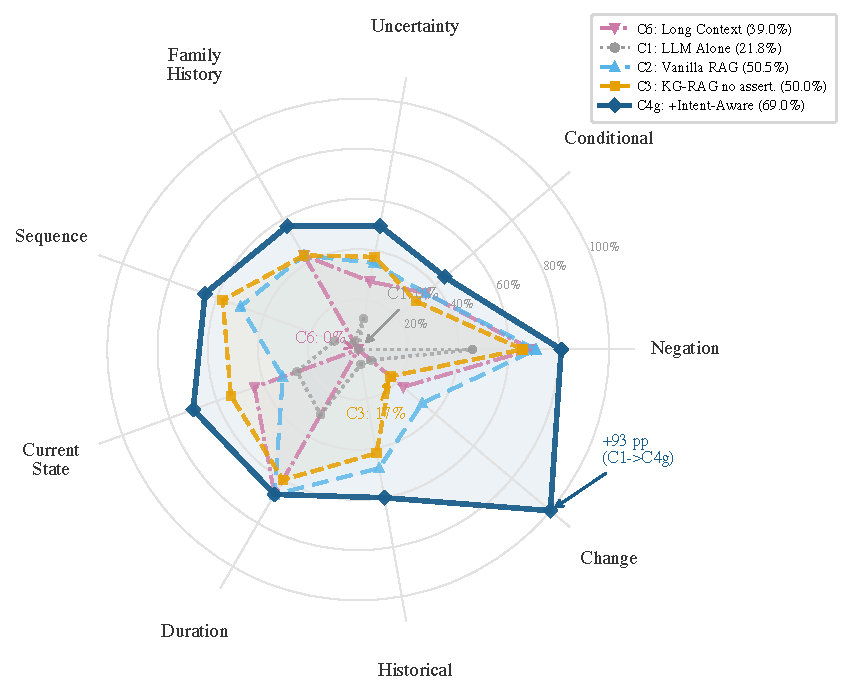
\includegraphics[width=\textwidth]{figures/fig2_radar.pdf}
\caption{ClinicalBench per-category accuracy across three conditions (C6, C1, C4g; Claude Opus 4.6, evaluator v2). C6 (pink dash-dot) collapses on historical and sequence (both 0\%); C1 (gray dotted) falls below 50\% on 7 of 9 categories, reflecting frequent abstentions without retrieval context; C4g (dark solid) improves all 9 categories over C1.}
\label{fig:radar}
\end{figure}

Table~\ref{tab:clinicalbench_categories} and Figure~\ref{fig:radar} reveal a strong \emph{category$\times$condition interaction}: intent-aware KG-RAG improves all 9 categories over C1, with every delta exceeding $+35\pp$.
Under the v2 evaluator with abstention detection, C1 drops sharply because the model without retrieval context frequently abstains (``insufficient information in the notes'') rather than attempting an answer.

\paragraph{Where intent-aware routing excels.}
\begin{sloppypar}
The largest gains occur on categories requiring cross-admission synthesis: change ($+83\pp$), sequence ($+55\pp$), historical ($+54\pp$), family history ($+53\pp$), conditional ($+45\pp$), and current state ($+44\pp$).
On the hard longitudinal subset (change + current state + historical, $n=130$), C4g outperforms C1 by $+56.9\pp$ (95\% BCa CI: \ci{+46.2\pp}{+65.4\pp}).
All nine category improvements exceed $+35\pp$ (Appendix Figure~\ref{fig:deltas}).
C6 fails catastrophically on historical (0\%) and sequence (0\%) despite Opus's 200K window, confirming that long context cannot substitute for structured retrieval on these categories.
\end{sloppypar}

% ----------------------------------------------------------
\subsection{Cross-Model Validation}
\label{sec:results:crossmodel}

\begin{table}[t]
\centering
\caption{ClinicalBench cross-model results (400 questions, keyword evaluator v2). All three models benefit from KG-RAG; the largest gain accrues to the most capable general-purpose model.}
\label{tab:crossmodel}
\small
\begin{tabular}{@{}llccl@{}}
\toprule
& Model & C1 & C4g & $\Delta$ \\
\midrule
Commercial & Claude Opus 4.6 & 22.5\% & \textbf{69.0\%} & $+46.5\pp$ \\
Open & GPT-OSS 20B & 20.8\% & 59.2\% & $+38.5\pp$ \\
Medical & MedGemma 27B & 26.5\% & 58.1\% & $+31.6\pp$ \\
\bottomrule
\end{tabular}
\end{table}

All three models benefit substantially from KG-RAG (Table~\ref{tab:crossmodel}), with the magnitude inversely related to parametric medical knowledge.
Opus gains $+46.5\pp$, GPT-OSS gains $+38.5\pp$, and MedGemma---the only model fine-tuned on medical corpora---gains $+31.6\pp$.
Notably, MedGemma starts with the highest C1 baseline (26.5\%) yet achieves the lowest C4g accuracy (58.1\%), while Opus starts at 22.5\% but reaches 69.0\% with retrieval.

All three models improve on all 9 categories under C4g (per-category cross-model breakdowns in Appendix Table~\ref{tab:crossmodel_categories}).
Intent-aware KG-RAG thus functions as a \emph{medical knowledge compensator}: the structured epistemic context partially substitutes for parametric medical knowledge, providing the largest benefit to general-purpose models that need it most.

% ----------------------------------------------------------
\subsection{SliceBench}
\label{sec:results:slicebench}

\begin{table}[t]
\centering
\caption{SliceBench overall results (144 questions, Claude Sonnet 4.5, judged by Opus 4.6). Sig: * denotes CI excluding zero.}
\label{tab:slicebench_overall}
\small
\begin{tabular}{@{}llccc@{}}
\toprule
& Condition & Score & 95\% CI & $\Delta$ vs B0 \\
\midrule
B0 & LLM Alone & 49.9\% & \ci{43.6\%}{56.1\%} & --- \\
B1 & Latest Note & 73.4\% & \ci{67.8\%}{78.7\%} & $+23.5\pp$ \\
B2 & All Notes RAG & 84.7\% & \ci{80.2\%}{88.8\%} & $+34.8\pp$ * \\
B3 & KG-RAG & 86.9\% & \ci{82.8\%}{90.8\%} & $+37.0\pp$ * \\
B4 & Full System & 87.6\% & \ci{83.7\%}{91.2\%} & $+37.8\pp$ * \\
\bottomrule
\end{tabular}
\end{table}

The incremental KG layer (B2$\rightarrow$B3) contributes $+2.2\pp$ overall (CI: \ci{-1.5\pp}{+5.9\pp}), not reaching aggregate significance, but tier-stratified estimates show a complexity-dependent trend: $+0.6\pp$ (Tier~A), $+1.0\pp$ (Tier~B), $+5.0\pp$ (Tier~C, 15+ encounters), consistent with KG context being most valuable when document volume overwhelms chunk-level retrieval (Appendix~\ref{app:slicebench_tiers}).

% ----------------------------------------------------------
\subsection{Physician Adjudication}
\label{sec:results:physician}

A two-physician blinded adjudication ($n=168$ questions $\times$ 2 conditions, Cohen's $\kappa$ for inter-rater reliability) is preregistered to validate automated scoring; the protocol (Appendix~\ref{app:physician_protocol}) was designed before examining results. \emph{Results are pending.}


% ============================================================
% 6. DISCUSSION & LIMITATIONS
% ============================================================
\section{Discussion and Limitations}
\label{sec:discussion}
% Section 6: Discussion and Limitations
% NOTE: \section{Discussion and Limitations} and \label{sec:discussion} are in main.tex

\paragraph{Why vanilla RAG hurts.}
Clinical notes contain dense negated, uncertain, and historical findings.
When vanilla RAG retrieves ``patient denies diabetes,'' the word ``diabetes'' enters context without the epistemic frame distinguishing absence from presence, actively misleading the model.
The C2~$<$~C1 finding (Table~\ref{tab:clinicalbench_ablation}) is consistent with GraphRAG-Bench~\cite{graphragbench2026}, which reports that GraphRAG underperforms when graph structure fails to encode task-relevant semantics---here, assertion status.

\paragraph{When KG context matters.}
The complexity-dependent Slice Bench effect (Tier~C: $+5.0\pp$ vs.\ Tier~A: $+0.6\pp$) suggests structured epistemic context is most valuable when: (a)~document volume overwhelms chunk-level retrieval, (b)~questions require cross-encounter synthesis where the same concept appears with different assertion states, and (c)~assertion status evolves across encounters.
For simple patients with few notes, the LLM tracks assertion context within retrieved chunks and the KG adds little.

\paragraph{Limitations.}
Sample size is modest: Slice Bench covers 6 patients (144 questions) and ClinicalBench covers 45 scenarios (400 questions), both from MIMIC-IV~\cite{johnson2023mimiciv}.
The overall B2$\rightarrow$B3 CI crosses zero (\ci{-1.5\pp}{+5.9\pp}), though the effect reaches practical significance within Tier~C.
Calculator/guideline integration (C5, B4) showed degradation attributable to component interaction effects when non-relevant modules activate, motivating query-aware component selection.
LLM-as-judge evaluation may introduce biases; our human validation by two board-certified physicians (blinded adjudication with inter-rater agreement) is reported in Appendix~\ref{app:human} and revealed overly strict automated scoring on uncertainty and sequence categories.
The majority of experiments use Claude, with cross-model validation (MedGemma 27B) covering only ClinicalBench.

\paragraph{Future work.}
Three directions follow: (1)~query-aware component selection to address C5/B4 degradation, (2)~expanding Tier~C to 20+ patients for sufficient statistical power, and (3)~systematic multi-model validation across open-source medical LLMs.


% ============================================================
% REFERENCES
% ============================================================
\bibliography{references}

% ============================================================
% APPENDIX (supplementary, not counted in 9-page limit)
% ============================================================
\newpage
\appendix
% ============================================================
% APPENDIX
% ============================================================

\section{Formal Epistemic Preservation}
\label{app:formal}

We formalize the epistemic invariant maintained by the \epikg pipeline, building on the principle that aboutness---the relationship between information artifacts and the entities they represent---must be preserved across transformations~\cite{ceusters2015ontologyepistemology}.

\begin{definition}[Epistemic State]
\label{def:epistemic}
For a clinical mention $m$, the \emph{epistemic state} is the tuple $e(m) = (c, \alpha, \xi, \tau)$, where $c$ is the OMOP concept identifier, $\alpha \in \mathcal{A}$ is the 7-value assertion label (Eq.~\ref{eq:assertion}), $\xi \in \{\textsc{Patient}, \textsc{Family}\}$ is the experiencer, and $\tau \in \{\textsc{Current}, \textsc{Past}, \textsc{Future}\}$ is the temporality.
A pipeline $P$ \emph{epistemically preserves} mention $m$ if $P(e(m)) = e(m)$; that is, the epistemic state at the output of every pipeline stage is identical to the state at extraction.
\end{definition}

\begin{proposition}[Assertion Entropy Loss]
\label{prop:entropy}
For concept $c$ in patient $\pi$'s record, let $A_c^\pi$ denote the assertion distribution with empirical frequencies $p(\alpha_i) = n_i / \sum_j n_j$ over the $|\mathcal{A}|$ assertion classes.
The assertion entropy is
\begin{equation}
\label{eq:entropy}
H(A_c^\pi) = -\sum_{i} p(\alpha_i) \log p(\alpha_i) \;.
\end{equation}
An assertion-blind pipeline collapses all mentions to $\alpha = \textsc{Present}$, yielding a degenerate distribution with $H = 0$.
The information loss is $\Delta H = H(A_c^\pi) \geq 0$~\cite{shannon1948}, with $\Delta H > 0$ strictly whenever any mention carries a non-present assertion.
\end{proposition}

\begin{corollary}[Faithfulness Bound]
\label{cor:faithfulness}
Let $f_{\textit{np}}(c)$ denote the fraction of mentions of concept $c$ carrying a non-present assertion ($\alpha \neq \textsc{Present}$).
Without assertion labels, the maximum assertion-faithful accuracy for any downstream task conditioned on $c$ is bounded by $1 - f_{\textit{np}}(c)$.
In clinical records where negated and uncertain mentions are prevalent---\eg ``no pneumonia,'' ``possible CHF''---this bound can be substantially below 1.
\end{corollary}


\section{Gap Analysis}
\label{app:gap}

\begin{table}[ht]
\centering
\caption{Capability comparison across representative systems. \smark{} = supported, $\circ$ = partial, \xmark{} = not supported.}
\label{tab:gap}
\small
\setlength{\tabcolsep}{3.0pt}
\begin{tabular}{@{}lcccccccc@{}}
\toprule
\textbf{System} & \rotatebox{70}{\textbf{Patient KG}} & \rotatebox{70}{\textbf{OMOP mapping}} & \rotatebox{70}{\textbf{Assertion (7-class)}} & \rotatebox{70}{\textbf{Tri-temporal}} & \rotatebox{70}{\textbf{Assert.-aware RAG}} & \rotatebox{70}{\textbf{Experiencer}} & \rotatebox{70}{\textbf{Allen's algebra}} & \rotatebox{70}{\textbf{Multi-hop ($\geq$3)}} \\
\midrule
DoctorRAG~\cite{lu2025doctorrag}         & \xmark & \xmark & \xmark & \xmark & \xmark & \xmark & \xmark & \xmark \\
GFM-RAG~\cite{luo2025gfmrag}             & $\circ$ & \xmark & \xmark & \xmark & \xmark & \xmark & \xmark & \smark{} \\
MedRAG~\cite{wang2025medrag}              & $\circ$ & \xmark & \xmark & \xmark & \xmark & \xmark & \xmark & $\circ$ \\
KARE~\cite{jiang2025kare}                 & $\circ$ & \xmark & \xmark & \xmark & $\circ$ & \xmark & \xmark & \smark{} \\
Multi-LLM KG~\cite{chen2026multilllmkgrag} & \xmark & \smark{} & $\circ$ & \xmark & \xmark & \xmark & \xmark & \xmark \\
MedTKG~\cite{huang2024medtkg}             & \smark{} & \xmark & \xmark & $\circ$ & \xmark & \xmark & \xmark & \smark{} \\
Graphiti~\cite{ramirez2025graphiti}       & \xmark & \xmark & \xmark & $\circ$ & \xmark & \xmark & \xmark & \smark{} \\
\midrule
\textbf{\epikg (ours)}                    & \smark{} & \smark{} & \smark{} & \smark{} & \smark{} & \smark{} & \smark{} & $\circ$ \\
\bottomrule
\end{tabular}
\end{table}

Partial marks indicate limited coverage: GFM-RAG, MedRAG, and KARE build population-level or hierarchical KGs (not per-patient longitudinal graphs); KARE uses KG-augmented retrieval but without assertion awareness; Multi-LLM KG models uncertainty via entropy but not the full assertion taxonomy; MedTKG and Graphiti use temporal annotations but not tri-temporal models.
\epikg's partial mark on multi-hop traversal ($\geq 3$ hops) reflects a deliberate architectural trade-off: PostgreSQL CTE-based traversal provides ACID compliance but degrades beyond 2~hops (Appendix~\ref{app:drknows}).


\section{Safety Score}
\label{app:safety}

The safety score $S = 1 - \frac{1}{N} \sum_{i=1}^{N} w_i \cdot \mathbb{1}[\hat{y}_i \neq y_i]$ applies $w_i = 2.0$ for false-positive assertion errors (reporting a negated or absent condition as present) and $w_i = 1.0$ otherwise, capturing asymmetric clinical risk where acting on a falsely affirmed condition is more dangerous than missing a present one.
We treat $w=2.0$ as a reasonable default; sensitivity to this choice is a direction for future work.


\section{Cross-Model Per-Category Results}
\label{app:crossmodel_categories}

\begin{table}[ht]
\centering
\caption{ClinicalBench per-category accuracy (\%) by model under C4 (epistemic KG-RAG). Epistemic evidence helps both models on assertion-dependent categories but hurts where the baseline is already strong.}
\label{tab:crossmodel_categories}
\small
\begin{tabular}{@{}lccccccc@{}}
\toprule
& & \multicolumn{3}{c}{MedGemma 27B} & \multicolumn{3}{c}{Claude Opus 4.6} \\
\cmidrule(lr){3-5} \cmidrule(lr){6-8}
Category & $n$ & C1 & C4 & $\Delta$ & C1 & C4 & $\Delta$ \\
\midrule
Negation & 110 & 100.0 & 100.0 & $=$ & 96.4 & 99.1 & \up{2.7} \\
Conditional & 20 & 100.0 & 70.0 & \dn{30.0} & 80.0 & 65.0 & \dn{15.0} \\
Uncertainty & 40 & 37.5 & 57.5 & \up{20.0} & 47.5 & 55.0 & \up{7.5} \\
Family hist. & 30 & 0.0 & 70.0 & \up{70.0} & 83.3 & 73.3 & \dn{10.0} \\
Sequence & 40 & 80.0 & 87.5 & \up{7.5} & 97.5 & 95.0 & \dn{2.5} \\
Current st. & 50 & 64.0 & 54.0 & \dn{10.0} & 58.0 & 48.0 & \dn{10.0} \\
Duration & 30 & 100.0 & 83.3 & \dn{16.7} & 90.0 & 100.0 & \up{10.0} \\
Historical & 50 & 94.0 & 60.0 & \dn{34.0} & 44.0 & 38.0 & \dn{6.0} \\
Change & 30 & 0.0 & 3.3 & \up{3.3} & 23.3 & 13.3 & \dn{10.0} \\
\midrule
\textbf{Overall} & \textbf{400} & \textbf{71.5} & \textbf{71.5} & $=$ & \textbf{72.5} & \textbf{70.2} & \dn{\textbf{2.2}} \\
\bottomrule
\end{tabular}
\end{table}


\section{Experiencer Attribute Propagation Ablation}
\label{app:experiencer}

The \texttt{experiencer} attribute distinguishes patient conditions from family member conditions; without it, the graph conflates the two, causing family history misattribution.

\begin{table}[ht]
\centering
\caption{Impact of experiencer attribute propagation on Opus C4 (400 questions, same C1 baseline of 72.5\%). Categories with no change omitted.}
\label{tab:experiencer_fix}
\small
\begin{tabular}{@{}lccc@{}}
\toprule
Category & Pre-fix & Post-fix & $\Delta$ \\
\midrule
Family history & 63.3\% & \textbf{73.3\%} & $+10.0\pp$ \\
Uncertainty & 50.0\% & \textbf{55.0\%} & $+5.0\pp$ \\
Historical & 34.0\% & 38.0\% & $+4.0\pp$ \\
Current state & 46.0\% & 48.0\% & $+2.0\pp$ \\
\midrule
\textbf{Overall C4} & \textbf{68.2\%} & \textbf{70.2\%} & $+2.0\pp$ \\
C4 vs C1 gap & $-4.2\pp$ & $-2.2\pp$ & gap halved \\
\bottomrule
\end{tabular}
\end{table}

The fix improved family history by $+10.0\pp$ with zero regressions on guard categories (negation, conditional, duration, sequence all unchanged), confirming that the experiencer attribute is load-bearing for assertion-sensitive reasoning.


\section{SliceBench Figures}
\label{app:slicebench_figures}

\begin{figure}[ht]
\centering
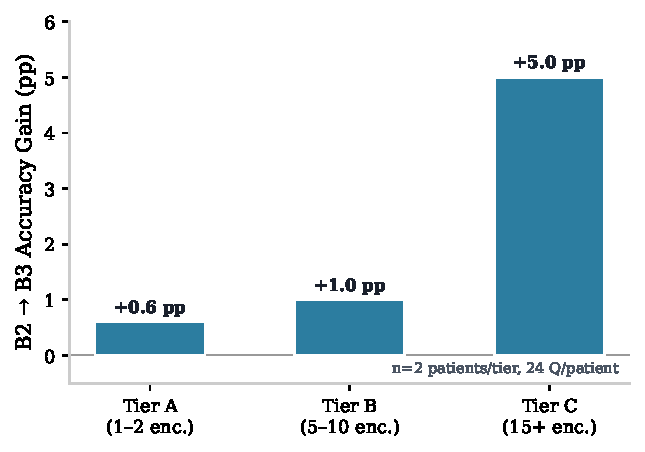
\includegraphics[width=0.75\textwidth]{figures/fig3_complexity_bars.pdf}
\vspace{4pt}
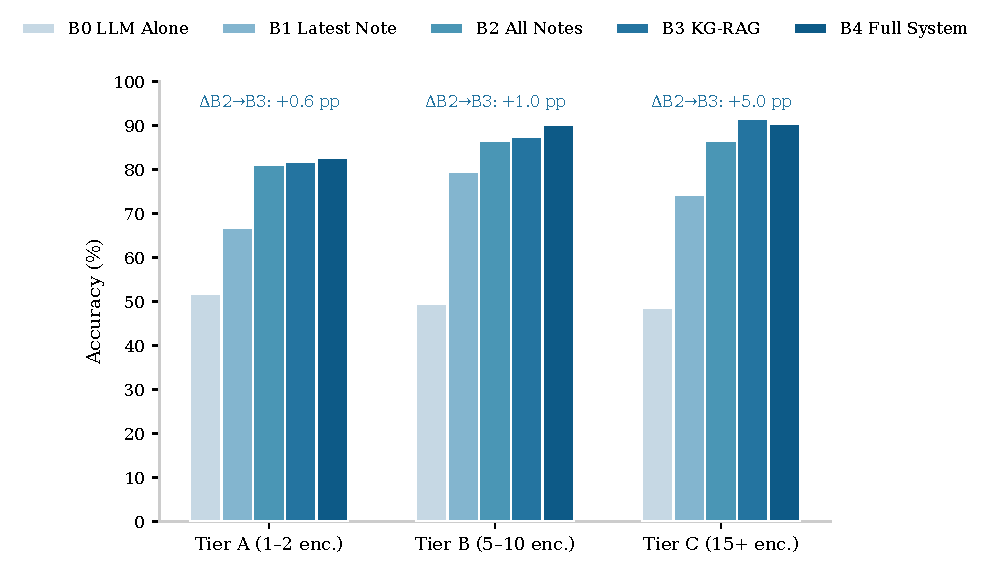
\includegraphics[width=\textwidth]{figures/fig4_waterfall.pdf}
\caption{SliceBench results ($n=2$ patients per tier, 24 questions each; point estimates without per-tier CIs). \textbf{Top:}~The KG layer's incremental benefit (B2$\rightarrow$B3) shows a directional, complexity-dependent trend: $+0.6\pp$ (Tier~A) to $+5.0\pp$ (Tier~C). \textbf{Bottom:}~Full condition progression by tier. The overall B2$\rightarrow$B3 delta is $+2.2\pp$ (CI: \ci{-1.5\pp}{+5.9\pp}).}
\label{fig:slicebench_figures}
\end{figure}


\section{Per-Category Delta Chart}
\label{app:deltas}

\begin{figure}[ht]
\centering
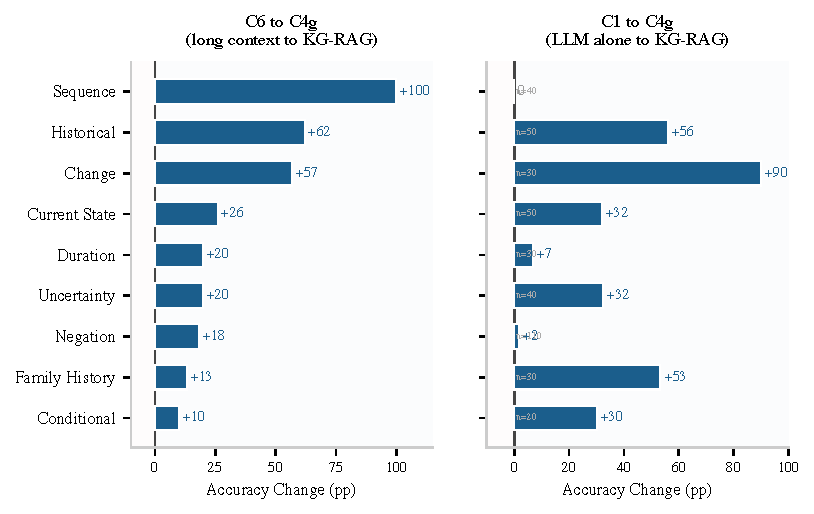
\includegraphics[width=\textwidth]{figures/fig5_category_deltas.pdf}
\caption{C1$\rightarrow$C4g per-category accuracy change. Intent-aware KG-RAG produces large gains on categories requiring cross-admission normalization (change, family history) and losses on categories where the LLM's parametric knowledge already suffices (historical, duration, conditional). Sample sizes per category shown.}
\label{fig:deltas}
\end{figure}


\section{SliceBench Conditions}
\label{app:slicebench_conditions}

\begin{table}[ht]
\centering
\small
\caption{SliceBench conditions. B0--B4 form a monotone context progression.}
\label{tab:slicebench_conditions}
\begin{tabular}{@{}clp{7.5cm}@{}}
\toprule
ID & Condition & Context Provided to LLM \\
\midrule
B0 & LLM Alone & Question only (parametric knowledge) \\
B1 & Latest Note & Most recent clinical note \\
B2 & All Notes RAG & All notes, retrieved by relevance \\
B3 & KG-RAG & Knowledge graph context + all notes \\
B4 & Full System & KG-RAG + guidelines + calculators \\
\bottomrule
\end{tabular}
\end{table}


\section{Supporting Results}
\label{app:supporting}

On MedQA-USMLE (965 questions), Claude Opus 4.5 achieves 81.6\% accuracy (5.1\,pp below GPT-4 at 86.7\% and Med-PaLM~2 at 86.5\%~\cite{medagentbench2025}), establishing that the Claude model family---Sonnet 4.5 (SliceBench answerer) and Opus 4.6 (ClinicalBench cross-model, SliceBench judge)---provides a reasonable LLM baseline.
Graph traversal latency is sub-millisecond at current scale (3,100 nodes, 8,803 edges): 0.57\,ms (1-hop), 0.75\,ms (2-hop).
The full system integrates 201 calculators, 1,202 guideline sections, 101 trigger patterns, and 24 edge types across 13 node types.


\section{DR.KNOWS Benchmark Results}
\label{app:drknows}

We evaluate \epikg on the DR.KNOWS diagnostic reasoning benchmark~\cite{drknows2025}, which measures knowledge graph traversal accuracy using real PostgreSQL-backed clinical data.

\begin{table}[ht]
\centering
\small
\begin{tabular}{lcc}
\toprule
\textbf{Metric} & \textbf{Score} & \textbf{\% of Baseline} \\
\midrule
Overall & 0.420 & 49.7\% \\
Path Discovery & 44.4\% & --- \\
Reasoning Accuracy & 22.2\% & --- \\
1-hop Traversal & 50.0\% & --- \\
2-hop Traversal & 25.0\% & --- \\
3-hop Traversal & 0.0\% & --- \\
\bottomrule
\end{tabular}
\caption{DR.KNOWS benchmark results. Multi-hop accuracy degrades due to PostgreSQL CTE limitations---an intentional tradeoff for ACID compliance.}
\label{tab:drknows}
\end{table}


\section{MedQA-USMLE Baseline}
\label{app:medqa}

\begin{table}[ht]
\centering
\small
\begin{tabular}{lccc}
\toprule
\textbf{Model} & \textbf{Accuracy} & \textbf{Step 1} & \textbf{N} \\
\midrule
EpiKG (LLM alone) & 81.6\% & 79.9\% & 965 \\
GPT-4 (2023) & 86.7\% & --- & 1{,}273 \\
Med-PaLM 2 (2023) & 86.5\% & --- & 1{,}273 \\
Claude 3 Opus (2024) & 78.0\% & --- & 1{,}273 \\
\bottomrule
\end{tabular}
\caption{MedQA-USMLE results. Our LLM-alone baseline is competitive.}
\label{tab:medqa}
\end{table}


\section{Scalability Metrics}
\label{app:scalability}

\begin{table}[ht]
\centering
\small
\begin{tabular}{lr}
\toprule
\textbf{Metric} & \textbf{Value} \\
\midrule
Documents processed & 145 \\
Patients & 85 \\
KG nodes & 3{,}100 \\
KG edges & 8{,}803 \\
1-hop traversal latency & 0.57\,ms \\
2-hop traversal latency & 0.75\,ms \\
\bottomrule
\end{tabular}
\caption{Scalability metrics at current deployment scale.}
\label{tab:scalability}
\end{table}


\section{System Component Scale}
\label{app:scale}

\begin{table}[ht]
\centering
\small
\begin{tabular}{lr}
\toprule
\textbf{Component} & \textbf{Scale} \\
\midrule
Clinical calculators & 201 \\
Guideline sections (RAG corpus) & 1{,}202 \\
OMOP vocabulary relationships & 20M+ \\
Assertion trigger patterns & 101 \\
KG edge types & 24 \\
KG node types & 13 \\
Assertion classes & 7 \\
\bottomrule
\end{tabular}
\caption{System component scale.}
\label{tab:system_scale}
\end{table}


\section{SliceBench Tier-Stratified Results}
\label{app:slicebench_tiers}

\begin{table}[ht]
\centering
\small
\caption{SliceBench results stratified by patient complexity tier. B2$\rightarrow$B3 $\Delta$ shows the incremental KG contribution.}
\label{tab:slicebench_tiers}
\begin{tabular}{@{}lccccccc@{}}
\toprule
& & \multicolumn{5}{c}{Score (\%)} & \\
\cmidrule(lr){3-7}
Tier & Encounters & B0 & B1 & B2 & B3 & B4 & B2$\rightarrow$B3 $\Delta$ \\
\midrule
A & 1--2 notes & 51.7 & 66.7 & 81.1 & 81.8 & 82.6 & $+0.6\pp$ \\
B & 5--10 notes & 49.5 & 79.4 & 86.4 & 87.4 & 90.1 & $+1.0\pp$ \\
C & 15+ notes & 48.4 & 74.2 & 86.5 & 91.5 & 90.3 & $+5.0\pp$ \\
\bottomrule
\end{tabular}
\end{table}


\section{ClinicalBench Full Per-Category Results}
\label{app:percategory}

\begin{table}[ht]
\centering
\small
\begin{tabular}{lcccccc}
\toprule
\textbf{Category} & \textbf{C1} & \textbf{C2} & \textbf{C3} & \textbf{C4} & \textbf{C4g} & \textbf{C5} \\
\midrule
Negation & 100.0 & 93.6 & 81.8 & 100.0 & 86.4 & 98.2 \\
Conditional & 100.0 & 90.0 & 55.0 & 70.0 & 65.0 & 75.0 \\
Uncertainty & 37.5 & 2.5 & 7.5 & 57.5 & 32.5 & 40.0 \\
Family History & 0.0 & 0.0 & 53.3 & 70.0 & 56.7 & 56.7 \\
Sequence & 80.0 & 80.0 & 80.0 & 87.5 & 90.0 & 77.5 \\
Current State & 64.0 & 54.0 & 50.0 & 54.0 & 76.0 & 58.0 \\
Duration & 100.0 & 100.0 & 83.3 & 83.3 & 46.7 & 73.3 \\
Historical & 94.0 & 78.0 & 68.0 & 60.0 & 40.0 & 68.0 \\
Change & 0.0 & 0.0 & 3.3 & 3.3 & 60.0 & 3.3 \\
\midrule
\textbf{Overall} & \textbf{71.5} & \textbf{62.5} & \textbf{59.2} & \textbf{71.5} & \textbf{66.0} & \textbf{68.2} \\
\bottomrule
\end{tabular}
\caption{Complete ClinicalBench per-category accuracy (\%, deterministic keyword evaluator) for all six conditions.}
\label{tab:full_percategory}
\end{table}


\section{Human Validation Pilot}
\label{app:human}

To assess LLM-as-judge reliability, we conducted a pilot validation study with a single board-certified physician who scored system outputs on a 4-point scale without knowledge of condition labels.
The pilot ($n=5$) revealed overly strict automated scoring on uncertainty and sequence questions. Gold standards were fully correct in 3/5 cases; model answers were partially correct or better in 3/5 cases where the auto-scorer marked them incorrect.
A full two-physician blinded adjudication ($n \geq 30$) is planned but not yet complete.


\section{Reproducibility Details}
\label{app:reproducibility}

\paragraph{Models.} ClinicalBench main ablation: MedGemma 27B via Ollama with deterministic keyword evaluator. Cross-model: MedGemma 27B and Claude Opus 4.6 (claude-opus-4-20250514) with the same evaluator. SliceBench: Claude Sonnet 4.5 (claude-sonnet-4-5-20250929, answering), Claude Opus 4.6 (judging). Temperature 0 throughout.

\paragraph{Evaluation.} The keyword evaluator matches temporal and assertion keywords against gold-standard categories, strips echoed evidence preambles, and includes expanded uncertainty keywords (medical hedging terms).

\paragraph{Bootstrap.} $n=2{,}000$ resamples, seed 42, BCa method~\cite{efron1993bootstrap}.

\paragraph{Data.} De-identified MIMIC-IV clinical notes under PhysioNet Credentialed Health Data Use Agreement~(v1.5.0).

\paragraph{Compute.} ClinicalBench: $\sim$3.6h (single GPU); Opus cross-model: $\sim$20min (API); SliceBench: $\sim$2h (API).

\paragraph{Evaluator evolution.} Key refinements: (i)~substring to word-boundary matching, (ii)~evidence preamble stripping. All main-text numbers use the final version.


\section{Assertion Category Definitions}
\label{app:assertions}

\begin{table}[ht]
\centering
\small
\begin{tabular}{lp{6.5cm}l}
\toprule
\textbf{Assertion} & \textbf{Definition} & \textbf{Example} \\
\midrule
\textsc{present} & Condition currently affirmed & ``has diabetes'' \\
\textsc{absent} & Condition explicitly negated & ``denies chest pain'' \\
\textsc{possible} & Condition suspected, not confirmed & ``possible pneumonia'' \\
\textsc{conditional} & Contingent on specific circumstances & ``if febrile, start antibiotics'' \\
\textsc{hypothetical} & Discussed as a scenario & ``would need dialysis if\ldots'' \\
\textsc{family\_history} & Attributed to a family member & ``mother had breast cancer'' \\
\textsc{historical} & Previously true, not necessarily current & ``former smoker'' \\
\bottomrule
\end{tabular}
\caption{The 7-value assertion taxonomy, extending i2b2 by separating \textsc{historical} from \textsc{family\_history}.}
\label{tab:assertion_defs}
\end{table}


\section{Intent-Aware Routing Algorithm}
\label{app:routing}

The C4g classifier is rule-based, mapping questions to \textsc{Change}, \textsc{Current\_State}, \textsc{Historical}, or \textsc{Default} using keyword patterns (e.g., ``changed'', ``new since'' trigger \textsc{Change}).
For \textsc{Change}, edges are partitioned by \texttt{hadm\_id} and set differences computed. For \textsc{Current\_State}, edges are filtered to current validity and deduplicated. For \textsc{Historical}, edges with past temporality are augmented with admission-based inference. Default questions use the C4 pipeline.


\section{C5 Full System Methodology}
\label{app:c5}

C5 extends C4 with guideline retrieval (1{,}202 sections) and clinical calculators (201, \eg CHA$_2$DS$_2$-VASc, MELD).
C5 achieves 68.2\% overall, below C1 and C4 (71.5\% each), likely because non-relevant components dilute the context window.


\section{Ethics Statement}
\label{app:ethics}

This work uses de-identified clinical data from MIMIC-IV~\cite{johnson2023mimiciv} under a PhysioNet Credentialed Health Data Use Agreement. No patient re-identification was attempted. The system is designed for clinical decision \emph{support}, not autonomous clinical decision-making.


% ============================================================
% NEURIPS PAPER CHECKLIST (mandatory)
% ============================================================
% NeurIPS Paper Checklist (mandatory)
% Do not remove this section.

\section*{NeurIPS Paper Checklist}

\begin{enumerate}

\item {\bf Claims}
    \item[] Question: Do the main claims made in the abstract and introduction accurately reflect the paper's contributions and scope?
    \item[] Answer: \answerYes{}
    \item[] Justification: The abstract and introduction state four specific contributions (Section~\ref{sec:intro}), each supported by empirical evidence in Sections~\ref{sec:results:clinicalbench}--\ref{sec:results:slicebench}. All claims include confidence intervals and are scoped with ``to our knowledge'' qualifiers where appropriate.

\item {\bf Limitations}
    \item[] Question: Does the paper discuss the limitations of the work performed by the authors?
    \item[] Answer: \answerYes{}
    \item[] Justification: Section~\ref{sec:discussion} explicitly discusses limitations including small sample sizes (6 patients for SliceBench, 2 per tier), single-site data (MIMIC-IV), the B2$\rightarrow$B3 confidence interval crossing zero, category-level trade-offs (C4 vs C1), and the ``change'' category capability gap.

\item {\bf Theory assumptions and proofs}
    \item[] Question: For each theoretical result, does the paper provide the full set of assumptions and a complete (correct) proof?
    \item[] Answer: \answerNA{}
    \item[] Justification: This is a systems paper with empirical evaluation; no theoretical proofs are claimed.

\item {\bf Experimental result reproducibility}
    \item[] Question: Does the paper fully disclose all the information needed to reproduce the main experimental results of the paper to the extent that it affects the main claims and/or conclusions of the paper?
    \item[] Answer: \answerYes{}
    \item[] Justification: Appendix~\ref{app:reproducibility} reports exact model versions (MedGemma 27B, Claude Sonnet 4.5, Claude Opus 4.6), temperature settings (0), bootstrap parameters ($n=2{,}000$, seed 42, BCa method), and data source (MIMIC-IV v1.5.0 under PhysioNet DUA). Section~\ref{sec:benchmarks} describes question generation and evaluation protocols.

\item {\bf Open access to data and code}
    \item[] Question: Does the paper provide open access to the data and code, with sufficient instructions to faithfully reproduce the main experimental results?
    \item[] Answer: \answerNo{}
    \item[] Justification: MIMIC-IV data is available under PhysioNet credentialed access (not open). Code will be released upon acceptance. Benchmark question templates and evaluation scripts will be included in the release.

\item {\bf Experimental setting/details}
    \item[] Question: Does the paper specify all the training and test details necessary to understand the results?
    \item[] Answer: \answerYes{}
    \item[] Justification: Section~\ref{sec:benchmarks} specifies benchmark design, question counts, condition definitions, patient selection criteria, and evaluation methodology. Appendix~\ref{app:reproducibility} provides model versions and computational requirements.

\item {\bf Experiment statistical significance}
    \item[] Question: Does the paper report error bars suitably and correctly?
    \item[] Answer: \answerYes{}
    \item[] Justification: Table~\ref{tab:slicebench_overall} reports BCa bootstrap 95\% CIs for all conditions. Per-tier results (Figure~\ref{fig:slicebench_figures}) are clearly labeled as point estimates without per-tier CIs due to small tier-level sample sizes ($n=2$ patients per tier). The overall B2$\rightarrow$B3 CI crossing zero is explicitly noted.

\item {\bf Experiments compute resources}
    \item[] Question: For each experiment, does the paper provide sufficient information on the computer resources needed to reproduce the experiments?
    \item[] Answer: \answerYes{}
    \item[] Justification: Appendix~\ref{app:reproducibility} reports computational requirements: ClinicalBench $\approx$3.6 hours (single GPU for MedGemma inference), SliceBench $\approx$2 hours (Anthropic API).

\item {\bf Code of ethics}
    \item[] Question: Does the research conducted in the paper conform, in every respect, with the NeurIPS Code of Ethics?
    \item[] Answer: \answerYes{}
    \item[] Justification: The study uses de-identified clinical data under an approved data use agreement (Appendix~\ref{app:ethics}). No patient re-identification was attempted. The system is designed for clinical decision \emph{support}, not autonomous decision-making.

\item {\bf Broader impacts}
    \item[] Question: Does the paper discuss both potential positive societal impacts and negative societal impacts of the work?
    \item[] Answer: \answerYes{}
    \item[] Justification: Section~\ref{sec:discussion} discusses the potential for improved clinical decision support (positive) and risks of over-reliance on automated systems, context dilution, and the need for physician oversight (negative). Appendix~\ref{app:ethics} addresses data ethics.

\item {\bf Safeguards}
    \item[] Question: Does the paper describe safeguards that have been put in place for responsible release of data or models?
    \item[] Answer: \answerYes{}
    \item[] Justification: The system operates on de-identified data under PhysioNet DUA. It is designed as a decision support tool requiring physician oversight. Code release will include usage guidelines emphasizing the system is not validated for autonomous clinical use.

\item {\bf Licenses for existing assets}
    \item[] Question: Are the creators or original owners of assets used in the paper properly credited and are the license and terms of use explicitly mentioned and properly respected?
    \item[] Answer: \answerYes{}
    \item[] Justification: MIMIC-IV is cited~\cite{johnson2023mimiciv} and used under PhysioNet Credentialed Health Data Use Agreement. All benchmark frameworks and models are cited. OMOP CDM is an open standard.

\item {\bf New assets}
    \item[] Question: Are new assets introduced in the paper well documented and is the documentation provided alongside the assets?
    \item[] Answer: \answerYes{}
    \item[] Justification: ClinicalBench and SliceBench are new benchmarks fully documented in Section~\ref{sec:benchmarks}, with question generation procedures, category definitions (Appendix~\ref{app:assertions}), and evaluation protocols. Templates and scoring scripts will accompany the code release.

\item {\bf Crowdsourcing and research with human subjects}
    \item[] Question: For crowdsourcing experiments and research with human subjects, does the paper include the full text of instructions given to participants and screenshots?
    \item[] Answer: \answerNA{}
    \item[] Justification: No crowdsourcing was used. Physician adjudication (Appendix~\ref{app:human}) involves expert review by co-authors, not human subjects research.

\item {\bf IRB approvals or equivalent}
    \item[] Question: Does the paper describe potential risks and does it include the IRB approval number if applicable?
    \item[] Answer: \answerNA{}
    \item[] Justification: MIMIC-IV is a de-identified public dataset; use under PhysioNet DUA does not require separate IRB approval per PhysioNet policy.

\end{enumerate}


\end{document}
